\documentclass[tikz,border=0pt]{standalone}
\begin{document}
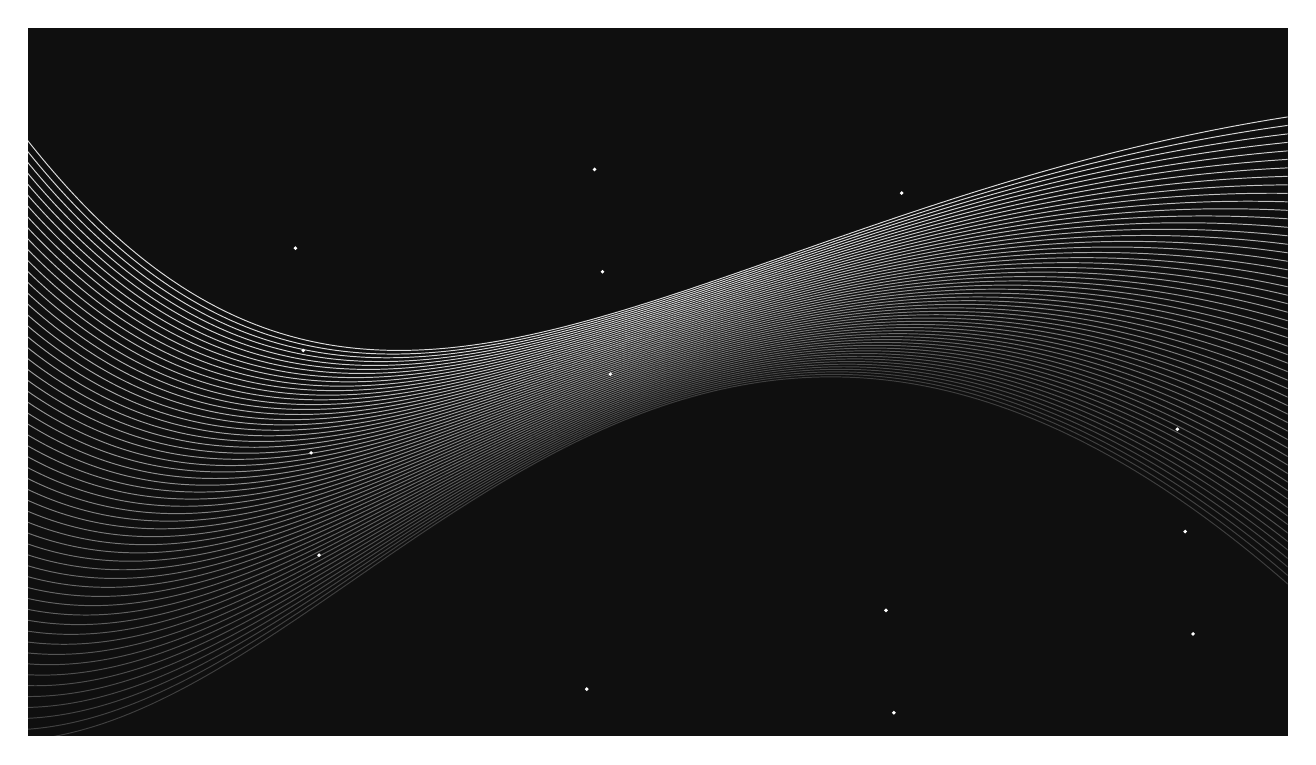
\begin{tikzpicture}
\fill[black!94] (0,0) rectangle (16,9);
\clip (0,0) rectangle (16,9);
\foreach \i in {0,...,55}{
  \pgfmathsetmacro{\a}{\i/55}
  \draw[white,opacity=.2+\a*.65,line width=.35pt]
  (-1,\a*9) .. controls (4,\a*2-1) and (8,10-\a*3) .. (17,\a*7+1);
}
\foreach \i in {1,...,14}{
  \pgfmathsetmacro{\x}{mod(\i*37,149)/10}
  \pgfmathsetmacro{\y}{mod(\i*23,79)/10}
  \fill[white] (\x,\y) circle (.025);
}
\end{tikzpicture}
\end{document}
